\subsection{Automating the Flow}
To enable rapid design-space exploration, we built an automated flow that integrates the components described in the previous sections.
Figure~\ref{fig_automating_flow_overview} summarizes the end-to-end tool flow discussed in this subsection.

\begin{figure}[t]
\centering
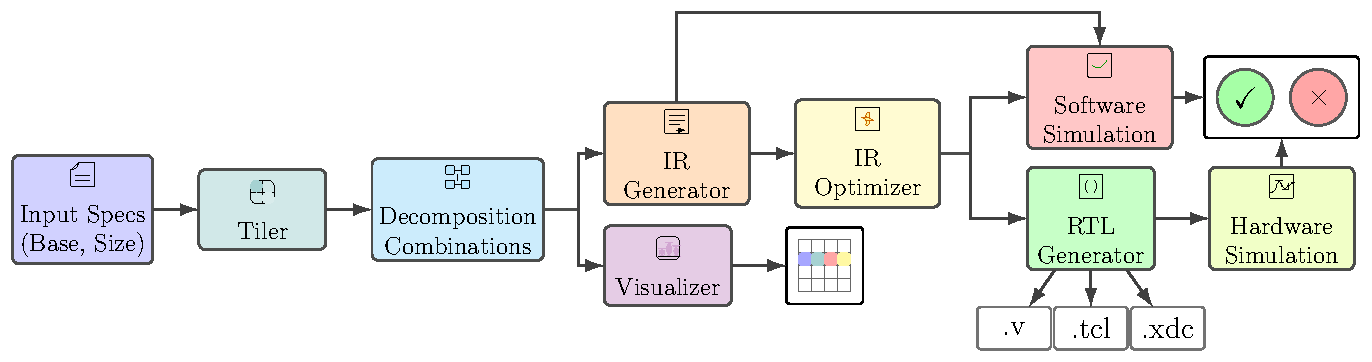
\includegraphics[width=\columnwidth]{figures/tool_explain/tool_overview_standalone.pdf}
\caption{Overview of the automated generation flow from specification to RTL and implementation reporting.}
\label{fig_automating_flow_overview}
\end{figure}

\noindent\textbf{Input Specification.}
The flow starts from a compact specification that includes the target multiplication size, base multiplier dimensions, desired decomposition strategy (Schoolbook, Karatsuba, or mixed), and the base combinational logic width.
This specification is architecture-aware: it captures enough information to guide both arithmetic decomposition and downstream hardware mapping.

\noindent\textbf{Tiler.}
The Tiler first instantiates a flat grid that covers the target multiplication using the selected base multiplier size.
When the target dimensions are not exact multiples of the base size, the remaining regions are filled using DSP block multipliers (Section~\ref{sec_tiler}), so full operand coverage is preserved.

\noindent\textbf{Hierarchy Generator.}
A single flat grid exposes limited structure for higher-level algebraic factoring.
The Hierarchy Generator therefore transforms the flat grid into alternative hierarchical decompositions by composing $2\times 2$ and $3\times 3$ groups at multiple levels.
For example, a flat $12\times 12$ grid can be rewritten as four $6\times 6$ blocks, where each $6\times 6$ block is itself decomposed into four $3\times 3$ bases, yielding three hierarchy levels (see Fig.~\ref{fig_target_constrained_tiling}).

\noindent\textbf{Exporter and Intermediate Representation (IR).}
Each decomposition variant is processed by the Exporter and Visualizer in parallel.
The Exporter emits an untimed intermediate representation (IR) that captures function, structure, and arithmetic intent before scheduling.
This IR follows the ArithV model: modules have explicit input/output interfaces, operations are represented as typed arithmetic nodes (e.g., add/sub/mul/shift/slice/concatenate), and each value carries explicit bit-width and signedness metadata.
The IR also preserves hierarchy and stable naming for generated submodules, marks DSP-fit primitive multipliers versus non-primitive multiplications requiring tiling, and records partial-product shift/alignment information used in later reduction stages.
Additionally, the IR carries software-level test intent so the same behavioral contract can be validated prior to RTL generation.
Because the IR is untimed, optimization passes can still apply algebraic rewrites, adder-tree balancing, and cascade-aware DSP grouping before clock-cycle decisions are made.

\noindent\textbf{IR Software Tester.}
The Software Tester executes the untimed IR in software simulation and compares outputs against the embedded test intent.
This catches arithmetic or decomposition errors early, reducing debug cost before RTL and implementation runs.

\noindent\textbf{Interpreter (Untimed Semantic Validation).}
After export, an interpreter executes the untimed IR semantics to validate function before hardware timing is introduced.
This stage resolves symbol bindings, evaluates arithmetic with explicit width/signedness rules, and checks slice/concatenate/shift behavior under the same semantics used in ArithV.
It executes the module-level test intent to ensure each generated decomposition variant is functionally correct at the software level.

\noindent\textbf{IR Optimization Passes.}
Starting from interpreter-validated IR, the toolchain applies optimization and lowering passes that preserve arithmetic equivalence while preparing for efficient hardware mapping.
Key passes include variable-version normalization to single-assignment form, DSP primitive recognition, DSP-chain grouping by shift/alignment constraints, decomposition of non-primitive multiplications via tiling, and accumulation rewriting into balanced or carry-save-oriented adder trees.
Target-specific legality checks are then applied (e.g., architecture-dependent cascade/shift constraints), producing an optimized untimed IR with explicit resource intent for RTL lowering.

\noindent\textbf{Visualizer.}
The Visualizer renders each decomposition as a layout/graph view and checks geometric correctness, including 100\% coverage and zero overlap constraints.
This stage provides an immediate sanity check for decomposition legality before hardware-specific transformations proceed.



\noindent\textbf{RTL Generator.}
After software validation, the RTL Generator lowers the optimized IR into timed, synthesizable Verilog modules and submodules.
At this stage, operation scheduling, pipelining, and synchronization are introduced according to the architecture-aware rules from Section~\ref{sec_build_base_mult} and Section~\ref{sec_fast_pipelined_comb_logic}, and testbenches are emitted for functional verification.

\noindent\textbf{Implementation and Reporting.}
Finally, the flow generates Tcl scripts to run FPGA synthesis/implementation and collect area/timing metrics.
It also emits annotated dataflow diagrams that indicate operation grouping and pipeline synchronization points, enabling direct correlation between algorithmic structure and hardware results.
%%%%%%%%%%%%%%%%%%%%%%%%%%%%%%%%%%%%%%%%%